

\tikzset{every picture/.style={line width=0.75pt}} %set default line width to 0.75pt        

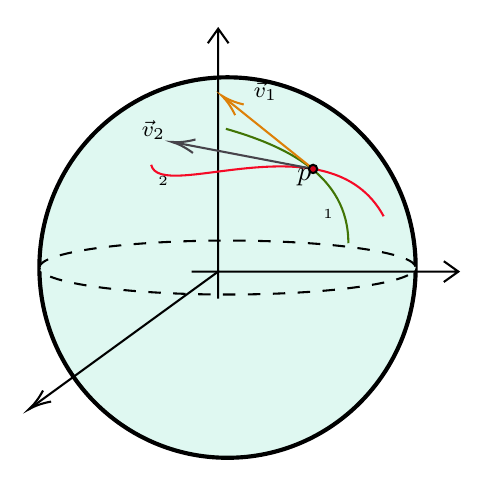
\begin{tikzpicture}[x=0.75pt,y=0.75pt,yscale=-1,xscale=1]
%uncomment if require: \path (0,256); %set diagram left start at 0, and has height of 256

%Shape: Ellipse [id:dp8621922183495604] 
\draw  [fill={rgb, 255:red, 223; green, 248; blue, 241 }  ,fill opacity=1 ][line width=1.5]  (205.14,135.71) .. controls (205.14,85.08) and (245.73,44.05) .. (295.79,44.05) .. controls (345.85,44.05) and (386.43,85.08) .. (386.43,135.71) .. controls (386.43,186.33) and (345.85,227.37) .. (295.79,227.37) .. controls (245.73,227.37) and (205.14,186.33) .. (205.14,135.71) -- cycle ;
%Shape: Ellipse [id:dp2859403935407516] 
\draw  [fill={rgb, 255:red, 223; green, 248; blue, 241 }  ,fill opacity=1 ][dash pattern={on 4.5pt off 4.5pt}] (205.14,135.71) .. controls (205.14,128.53) and (245.73,122.71) .. (295.79,122.71) .. controls (345.85,122.71) and (386.43,128.53) .. (386.43,135.71) .. controls (386.43,142.89) and (345.85,148.71) .. (295.79,148.71) .. controls (245.73,148.71) and (205.14,142.89) .. (205.14,135.71) -- cycle ;
%Shape: Axis 2D [id:dp5781161322417953] 
\draw  (278.43,137.66) -- (407,137.66)(291.29,20.64) -- (291.29,150.66) (400,132.66) -- (407,137.66) -- (400,142.66) (286.29,27.64) -- (291.29,20.64) -- (296.29,27.64)  ;
%Straight Lines [id:da986530720222472] 
\draw    (291.29,137.66) -- (201.62,202.87) ;
\draw [shift={(200,204.05)}, rotate = 323.97] [color={rgb, 255:red, 0; green, 0; blue, 0 }  ][line width=0.75]    (10.93,-3.29) .. controls (6.95,-1.4) and (3.31,-0.3) .. (0,0) .. controls (3.31,0.3) and (6.95,1.4) .. (10.93,3.29)   ;
%Curve Lines [id:da2567673398245671] 
\draw [color={rgb, 255:red, 245; green, 10; blue, 38 }  ,draw opacity=1 ]   (259,86.2) .. controls (263.29,105.12) and (345,63) .. (371,111) ;
%Curve Lines [id:da2661789837245453] 
\draw [color={rgb, 255:red, 65; green, 117; blue, 5 }  ,draw opacity=1 ]   (295,68.87) .. controls (323,76.87) and (354,90.87) .. (354,124) ;
%Straight Lines [id:da53165768173298] 
\draw [color={rgb, 255:red, 71; green, 68; blue, 75 }  ,draw opacity=1 ][fill={rgb, 255:red, 61; green, 57; blue, 57 }  ,fill opacity=1 ][line width=0.75]    (337,88.2) -- (270.96,75.58) ;
\draw [shift={(269,75.2)}, rotate = 10.82] [color={rgb, 255:red, 71; green, 68; blue, 75 }  ,draw opacity=1 ][line width=0.75]    (10.93,-3.29) .. controls (6.95,-1.4) and (3.31,-0.3) .. (0,0) .. controls (3.31,0.3) and (6.95,1.4) .. (10.93,3.29)   ;
%Straight Lines [id:da3674366892672871] 
\draw [color={rgb, 255:red, 221; green, 128; blue, 8 }  ,draw opacity=1 ][fill={rgb, 255:red, 61; green, 57; blue, 57 }  ,fill opacity=1 ][line width=0.75]    (337,88.2) -- (294.56,54.12) ;
\draw [shift={(293,52.87)}, rotate = 38.77] [color={rgb, 255:red, 221; green, 128; blue, 8 }  ,draw opacity=1 ][line width=0.75]    (10.93,-3.29) .. controls (6.95,-1.4) and (3.31,-0.3) .. (0,0) .. controls (3.31,0.3) and (6.95,1.4) .. (10.93,3.29)   ;
%Shape: Circle [id:dp7854098221379334] 
\draw  [fill={rgb, 255:red, 208; green, 2; blue, 27 }  ,fill opacity=1 ] (335,88.2) .. controls (335,87.1) and (335.9,86.2) .. (337,86.2) .. controls (338.1,86.2) and (339,87.1) .. (339,88.2) .. controls (339,89.3) and (338.1,90.2) .. (337,90.2) .. controls (335.9,90.2) and (335,89.3) .. (335,88.2) -- cycle ;

% Text Node
\draw (253,63.59) node [anchor=north west][inner sep=0.75pt]  [font=\footnotesize]  {$\vec{v}_{2}$};
% Text Node
\draw (340.43,106.05) node [anchor=north west][inner sep=0.75pt]  [font=\scriptsize]  {$\upsigma _{1} \ \ $};
% Text Node
\draw (261,90.6) node [anchor=north west][inner sep=0.75pt]  [font=\scriptsize]  {$\upsigma _{2} \ \ $};
% Text Node
\draw (307,44.59) node [anchor=north west][inner sep=0.75pt]  [font=\footnotesize]  {$\vec{v}_{1}$};
% Text Node
\draw (328,86.4) node [anchor=north west][inner sep=0.75pt]    {$p$};


\end{tikzpicture}
